\subsection{Power Saving for Major App Activities}
\label{subsec:activities}

% App selection based on popularity - top 10 app category
% Online social networking
% Messaging
% Streaming video
% Streaming music
% Power saving for each category

%  Popular Dark theme mode enabled Google Android Apps \cite{android_dark_app_list}

% are used to generate current consumption comparison between dark theme and light modes

From app developers' perspective, an app consists of multiple
activities, each implementing a user interface to interact
with the app. Hence, to add dark mode to an app, the developer's
effort largely boils down to implementing dark mode for each
activity. In this section, we show how to use the PFOP profiler to
gain insight into the power saving for the major activities in the set of Google
apps.

\paragraph{Methodology.}
We manually navigate each of the apps to stop at all its major
activities when running under dark mode and light mode, and run
the PFOP profiler to measure the display power draw.
In all, we studied 34 activities of the 6 apps, with
many app-specific findings.
% and capture the screen via screencap. We then apply our P-LMLR
% power model to the captured screens to calculate the power draw.
%   Table~\ref{tab:experiments} lists the activity instances used for the
%  set of Google apps studied in our experiment.
\if 0

\begin{table}[tp]
\begin{center}
	\centering
	\caption{Activities studied in the popular Google Apps.}
	\label{tab:experiments}
        \vspace{-0.1in}
	% \begin{tabular*}{\columnwidth}{@{\extracolsep{\fill}}| l | l |}
	\small {
	\begin{tabular*}{\columnwidth}{ | p{0.25\columnwidth} | p{0.665\columnwidth} | }
		\hline
		App Name        	& Activity\\
		\hline
		Calculator		& Home, Function Screen, History, Choose Theme, Typed Entry, Help, Current Expression \\
		Phone			& Home, Keypad, Type Number, New Contacts, Recent, Contacts, Settings, Favorites \\
		Google Calender		& Home, Days, Week, Month, Settings, Calender Dropdown, Help \\
		Google Maps		& Open Navigation, Search, Route \\  
		News			& Various sections \\
		YouTube			& Home, Trending, Subscription, Inbox, Library, Search, Video, No Connection\\
		GBoard 			& Google Keyboard \\
		Launcher        	& Launcher Activity \\
		SystemUI        	& Settings \\
		\hline
	\end{tabular*}
	}
\end{center}
\vspace{-0.15in}
\end{table}
\fi

\if 0
\subsubsection{Overall Results}

Table~\ref{tab:Dark_vs_light_popular_google_apps} shows the total
phone power measured using the built-in power sensor and the
% estimated
OLED display power output by the PFOP profiler
% using the power model for the major activities
for the set of Google and system apps on the 3 phones under light and dark mode,
under screen brightness 100\%.
We make the following observations.
(1) The total phone power in displaying the same app activities
differ across the three phones. The average phone power across all activities for all apps
in light mode are 347mA, 365mA, and 418mA, respectively, on the 3 phones.
(2) The major source of phone power draw difference for the same app activities
comes from the difference in OLED power draw;
the average OLED power across all activities of all apps
in light mode are 283mA, 282mA, and 386mA, respectively, on the 3 phones.
(3) Switching from light mode to dark mode significantly reduces the OLED power
draw of the app activities, ranging between 42\%--71\% (average 61\%),
33\%--88\% (average 76\%), and 31\%--79\% (average 68\%),
across the apps on the 3 phones, respectively.
(4) The drastic OLED power saving in switching to dark mode 
translates into significant saving of whole phone power draw,
on average 48\%, 52\%, and 56\% across the apps on the 3 phones, respectively.
\fi

\if 0
\begin{table}[tp]
	\centering
	\caption{Average total phone power and OLED power (mA) across major activities of popular
          Google apps under light and dark modes at brightness level 100\%.
            The Phone app is not supported on Moto Z3.}
        \vspace{-0.1in}
               {\small
               %\begin{tabular*}{\columnwidth}{@{\extracolsep{\fill}}| l | c | c | c | c |c|c|}
       \begin{tabular}{| l | c | c | c | c |c|c|}
		\hline
	& \multicolumn{2}{c |}{Light mode} & \multicolumn{2}{c |}{Dark mode}& \multicolumn{2}{c |}{Power reduction} \\
			\cline{2-7}
	App Name        & Total & OLED & Total & OLED & Total & OLED  \\
	\hline
         \multicolumn{7}{|c|}{Nexus 6} \\
         \hline
	 Calculator	&  323 &  291 &  125 &   93 &   61\% &   67\% \\
	 Phone		&  325 &  311 &  117 &   87 &   63\% &   71\% \\
         Calender	&  341 &  320 &  136 &   97 &   60\% &   69\% \\
	 Google Maps	&  430 &  273 &  324 &  120 &   24\% &   55\% \\
	 News		&  398 &  314 &  190 &  102 &   52\% &   67\% \\
	 YouTube	&  334 &  278 &  168 &  112 &   49\% &   59\% \\
	 GBoard		&  278 &  199 &  187 &  113 &   32\% &   42\% \\
	 \hline
         \multicolumn{7}{|c|}{Pixel 2} \\
         \hline
	 Calculator	&  324 &  279 &  111 &   39 &   65\% &   85\%  \\
	 Phone		&  349 &  313 &   97 &   35 &   72\% &   88\%  \\
	 Calender	&  355 &  313 &  118 &   47 &   66\% &   84\%  \\
	 Google Maps	&  377 &  223 &  225 &   44 &   40\% &   80\%  \\
	 News		&  370 &  312 &  143 &   47 &   61\% &   84\%  \\
	 YouTube	&  336 &  266 &  142 &   53 &   57\% &   80\%  \\
	 GBoard		&  361 &  299 &  297 &  200 &   17\% &   33\%  \\
	 Launcher       &  410 &  279 &  233 &   79 &   43\% &   71\%  \\
	 SystemUI       &  400 &  255 &  204 &   49 &   48\% &   80\%  \\
	 \hline
         \multicolumn{7}{|c|}{Moto Z3} \\
	 \hline
	 Calculator	&  401 &  393 &  126 &   78 &   68\% &   79\% \\
	 Calender	&  444 &  441 &  141 &   93 &   68\% &   78\% \\
	 Google Maps	&  425 &  327 &  195 &   86 &   54\% &   73\% \\
	 News		&  462 &  419 &  163 &   93 &   64\% &   77\% \\
	 YouTube	&  396 &  358 &  172 &  107 &   56\% &   70\% \\
	 GBoard		&  456 &  441 &  352 &  301 &   22\% &   31\% \\
	 Launcher       &  359 &  335 &  174 &  118 &   51\% &   64\% \\
	 SystemUI       &  397 &  378 &  136 &   88 &   65\% &   76\% \\
	 \hline
\end{tabular}
}
\label{tab:Dark_vs_light_popular_google_apps}
\end{table}
\fi

%  To gain insight into how UI designs affect the benefits from dark mode,
%
%   Since an app activity may consist of three
%   types of components, \ie text, rendered graphics, and
%   embedded objects (\eg images and videos)
%  The embedded objects usually contain
%  pre-generated  graphics contents that are non-modifiable and hence dark mode will
%  be less effective for the activities that are occupied with more
%  embedded objects. In the following,
One expected general finding is that
the power saving from switching to dark mode
correlates with the amount of embedded dynamic objects (\eg videos, ads):
the more pixels dynamic objects occupy, the less power savings, as they stay the same
in light and dark modes.
\if 0
We grouped the apps  into three categories according to
whether their main activities consist of embedded objects, with graphics rendering, or
with text only, and used \name to analyze how 
their OLED display power savings due to dark mode correlates
with the UI components.
\fi
Due to page limit, we will only present the case study for Google News.
% \subsubsection{Apps with Embedded Objects}

Google News
% and YouTube
represents the class of apps whose main
activities are rich in pre-generated graphical objects, such as images
(static) or videos (dynamic). Since the graphical objects typically
stay the same in light and dark mode, the OLED power saving of
such activities depends on the portion of the screen occupied by such
embedded objects.
% We discuss Google News below and leave detailed discussions about YouTube in Appendix A1. 

\begin{figure}[th]
	\begin{subfigure}[]{\columnwidth}
		\centering
		% \includegraphics[width=0.58\columnwidth]{./figure/609_news_light.pdf}\quad
		% \frame{\includegraphics[width=0.27\columnwidth]{./figure/659_news_light.png}}
		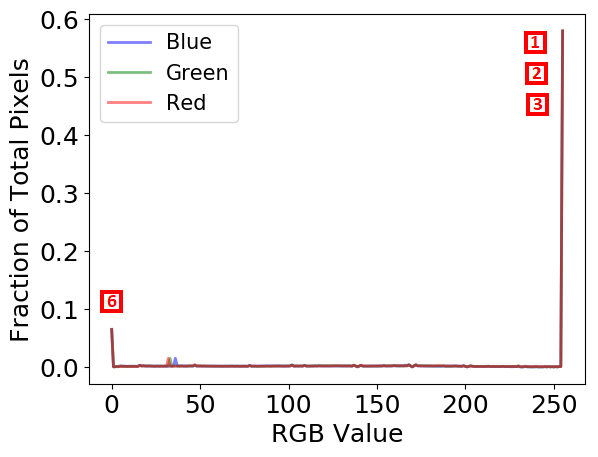
\includegraphics[width=0.58\columnwidth]{./figure/609a_news_light.png}\quad
		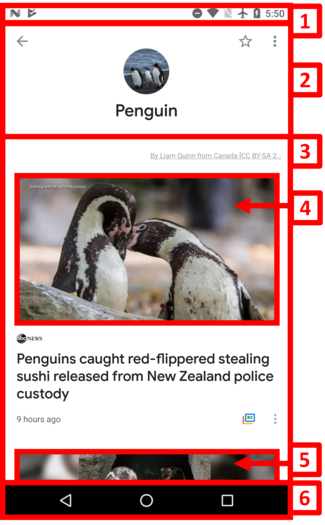
\includegraphics[width=0.27\columnwidth]{./figure/659a_news_light.png}
		\caption{PFOP output for light mode}
	\end{subfigure}
	\begin{subfigure}[]{\columnwidth}
		\centering
		% \includegraphics[width=0.58\columnwidth]{./figure/608_news_dark.pdf}\quad
		% \frame{\includegraphics[width=0.27\columnwidth]{./figure/658_news_dark.png}}
		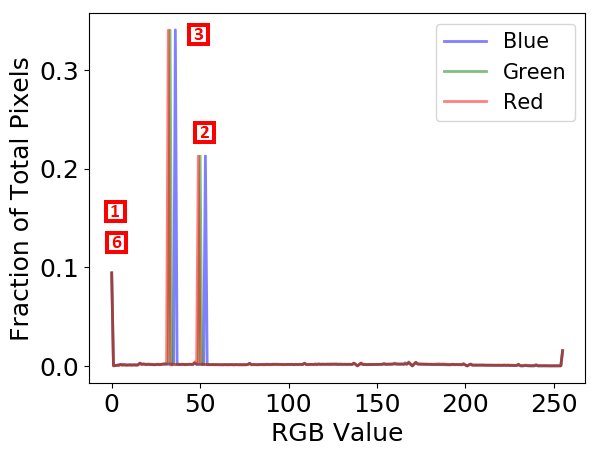
\includegraphics[width=0.58\columnwidth]{./figure/608a_news_dark.png}\quad
		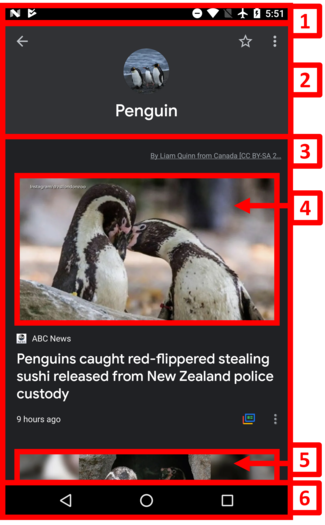
\includegraphics[width=0.27\columnwidth]{./figure/658a_news_dark.png}
		\caption{PFOP output for dark mode}
	\end{subfigure}
	% \\
	\begin{subfigure}[]{\columnwidth}
	\begin{subfigure}[]{0.42\columnwidth}
		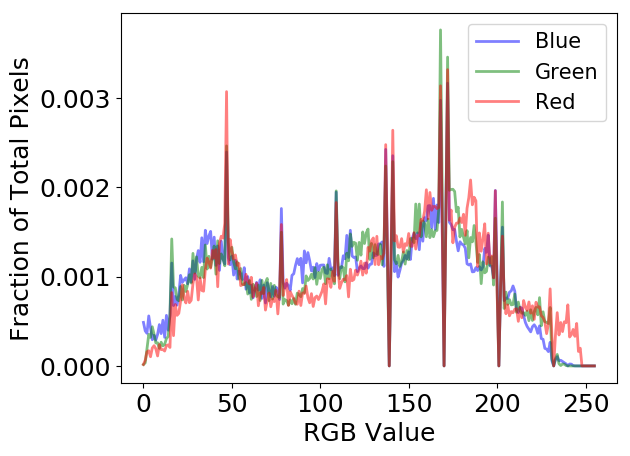
\includegraphics[width=\columnwidth]{./figure/692a_news_penguin.png}
		\caption{Pixel color histogram of the penguin image.}
		\label{fig:case_study_embedde_object}
	\end{subfigure}
	\begin{subfigure}[]{0.38\columnwidth}
	\centering
	{ \scriptsize
	\begin{tabular}{ | l | r | r | r | }
		\hline
		     & \multicolumn{3}{|c|}{Power Reduction (mA)}\\
		\cline{2-4}
                Part & Nexus 6 & Pixel 2 & Moto Z3 \\
		\hline
		1 &   6  &   8 &   10  \\
		2 &  46  &  59 &   77  \\
		3 &  78  &  97 &  129  \\
		4 &   0  &   0 &    0  \\
		5 &   0  &   0 &    0  \\
		6 &   0  &   0 &    0  \\
		\hline
		Total   & 130 & 164 & 216  \\
		\hline
	\end{tabular}
	}
	\caption{OLED power saving (from PFOP per-component output}		
	\end{subfigure}
        \vspace{-0.1in}
	\end{subfigure}
	\caption{Google News: Headlines activity.}
        \vspace{-0.20in}
	\label{fig:case_study_news}
\end{figure}

\if 0
\begin{figure}[th]
	\begin{subfigure}[]{\columnwidth}
		\centering
		% \includegraphics[width=0.58\columnwidth]{./figure/609_news_light.pdf}\quad
		% \frame{\includegraphics[width=0.27\columnwidth]{./figure/659_news_light.png}}
		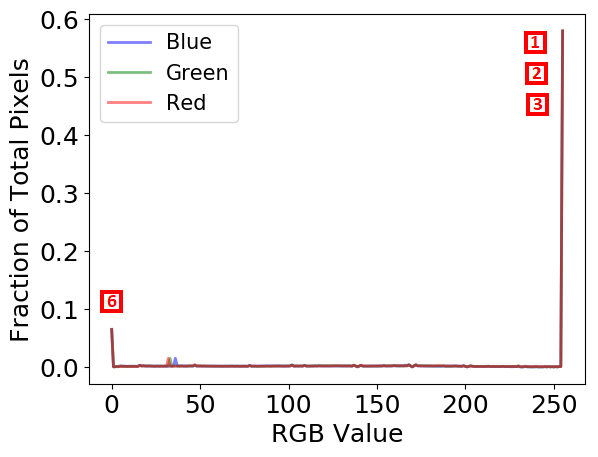
\includegraphics[width=0.58\columnwidth]{./figure/609a_news_light.png}\quad
		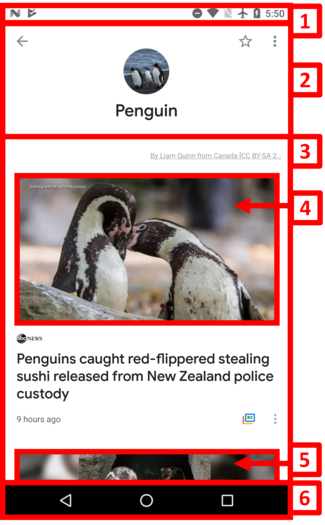
\includegraphics[width=0.27\columnwidth]{./figure/659a_news_light.png}
		\caption{PFOP output for Light mode}
	\end{subfigure}
	\begin{subfigure}[]{\columnwidth}
		\centering
		% \includegraphics[width=0.58\columnwidth]{./figure/608_news_dark.pdf}\quad
		% \frame{\includegraphics[width=0.27\columnwidth]{./figure/658_news_dark.png}}
		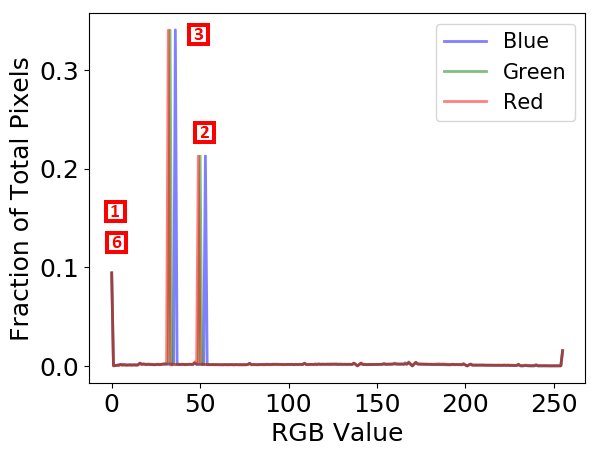
\includegraphics[width=0.58\columnwidth]{./figure/608a_news_dark.png}\quad
		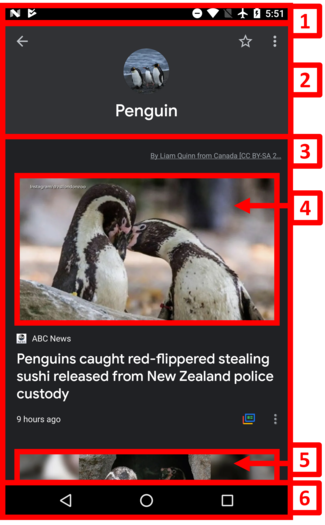
\includegraphics[width=0.27\columnwidth]{./figure/658a_news_dark.png}
		\caption{PFOP for Dark mode}
	\end{subfigure}
	\\
	\begin{subfigure}[]{\columnwidth}
	\centering
	{ \small
	\begin{tabular}{ | l | r | r | r | }
		\hline
		     & \multicolumn{3}{|c|}{Power Reduction (mA)}\\
		\cline{2-4}
                Part & Nexus 6 & Pixel 2 & Moto Z3 \\
		\hline
		1 &   6  &   8 &   10  \\
		2 &  46  &  59 &   77  \\
		3 &  78  &  97 &  129  \\
		4 &   0  &   0 &    0  \\
		5 &   0  &   0 &    0  \\
		6 &   0  &   0 &    0  \\
		\hline
		Total   & 130 & 164 & 216  \\
		\hline
	\end{tabular}
	}
	\caption{OLED power saving (from PFOP per-component output}		
        \vspace{-0.1in}
	\end{subfigure}
	\caption{Google News: Headlines activity.}
        \vspace{-0.20in}
	\label{fig:case_study_news}
\end{figure}

\begin{figure}[h]
	\begin{subfigure}[]{\columnwidth}
		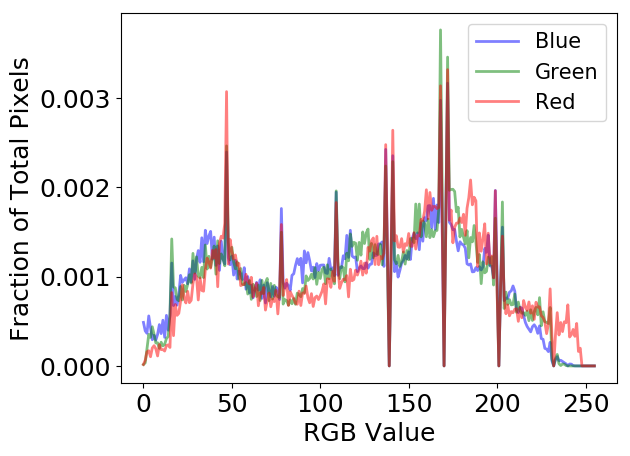
\includegraphics[width=0.58\columnwidth]{./figure/692a_news_penguin.png}\quad
		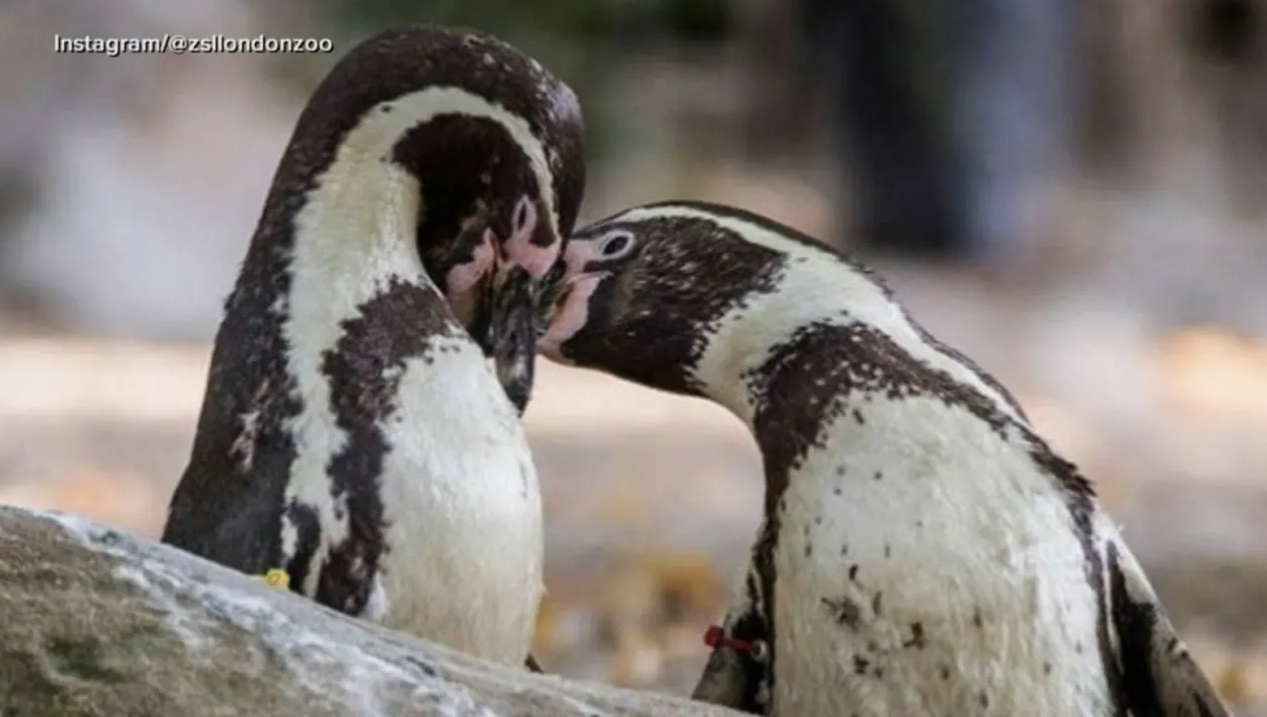
\includegraphics[width=0.27\columnwidth]{./figure/691_news_penguin.png}
	\end{subfigure}
	\caption{Pixel color histogram of the penguin image.}
        \vspace{-0.1in}
	\label{fig:case_study_embedde_object}
\end{figure}
\fi

% {\bf Google News.}
Figure~\ref{fig:case_study_news} shows the results
for the main activity of Google News.  The screen is dominated by
topic (part 2), news section (part 3), and embedded image (part 4).
The remaining sections, Status bar (part 1) and Navigation bar (part
6), are small.
% as usual.
Figure 12d shows the major OLED power saving in switching to dark mode comes from
part 2 and part 3 which switch from white color to near-dark color
(RGB values around 50).

As expected, the embedded image stays the same
in the two modes and contribute to no OLED power saving. 
The reason we do not see any obvious peak in the histogram that corresponds to
the image (24.9\% of the screen size) is that 
the image has continuous textures which make the histogram spread over
a wide range of RGB values, as shown in the enlarged pixel histogram of
the penguin image only in Figure~\ref{fig:case_study_embedde_object}.

\if 0
So even if the images cover a large area still we
can't observe any peaks. We extracted the penguin image from the Google News
app and  after analyzing it we observed that although total fraction of pixels
is about 25 \% of total pixels, the histogram is distributed for RGB range and
makes it obscure i.e in the full image histogram fraction of pixel value is not
perceivable.Total saving in dark theme Google News mode is about 132mA/167mA/221mA.
\fi


\if 0
like the Google News where the change in images RGB Histogram is not
perceivable as images are obscured due to continuous texture nature of
natural images. For YouTube app the status bar (1) and the upper section (2)
are similar to the News app and The saving in Dark theme mode is
6mA/6mA/8mA for (1) and for 15mA/18mA/24mA for (2). YouTube main body (3) has
the maximum saving in our study and the saving is about 120mA/151mA/200mA for (3).
The lower bar (5) in YouTube has two major aspects i.e change in background
color and the color of the icon which saves power. This is why there is shift
in the RGB histogram.The saving (5) is  13mA/17mA/22mA. Like most of the other
apps the Navigation bar (6) doesn't change color and hence there is no
savings.i.e saving value is 0mA/0mA/0mA for (6).
Total saving by dark mode for Google News app is 154mA/189mA/251mA.
\fi

% \subsection{Power saving for app run}
% 
% We used the UI Animator to run the app in light and dark model to observe
% effect of dark modes on the battery life.

\if 0
\subsubsection{Apps with Graphical Rendering}

{\bf Google Map.} This app represents the class of apps
whose activities are dominated with graphical rendering, including
AR, navigation, and music apps.
The
main activity is dominated
by the dynamically changing map (part 5),
consisting of roads and blocks which
change from white to dark grey in switching from the light to dark mode
and contribute to the majority of the OLED power saving.
Detailed discussions can be found in Appendix A1.
\fi


\if 0
is Green which doesn't change
with change of modes. These saves 0.2mA/0.2mA/0.2mA for (1),
0.8mA/0.8mA/1mA for (2) and 0.2mA/0.2mA/0.3mA for (3). The Navigation Bar (7)
is Black and is constant. It does not save (0mA/0mA/0mA). The side bar (4)
contains lot of buttons which changes to dark color.This saves
about 10mA/12mA/16mA. The body of the app is the trickiest. This contains
digital images and changes the color depending on the contents. For our
instance the saving is about 113mA/132mA/175mA for (5) and
24mA/31mA/41mA for (6).
\fi

\if 0
\subsubsection{Apps with Text Only}

Google Calculator, Google Calender and Google Phone activities contain
text only. Since the UI design n dark mode is relatively simple compared
to the next two categories,
we leave their detailed discussions in Appendix A1.
%due to page limit.
%  We observed how the dark theme mode is implemented for
%  these apps and estimated power saving for Nexus 6/Pixel 2/Moto Z3
%  phones.  From our findings parallel inference of power savings can be
%  drawn for other phones.

\fi



